\chapter{Sexual Reproduction of Flowering Plants}\label{ch:b2:angiosperm-reproduction}

An apple orchard in May is white with blossom and loud with bees;
in October the same trees are heavy with \omterm{def:b2:angiosperm-reproduction:seed}{fruit}, each apple holding
ten \omterm{def:b2:angiosperm-reproduction:seed}{seeds}, each \omterm{def:b2:angiosperm-reproduction:seed}{seed} an embryo tree wrapped in a store of food. The
whole of that transformation --- the \omterm{def:b2:angiosperm-reproduction:flower}{flower}, the \omterm{def:b2:plant-life-cycles:heterospory}{pollen} carried by an
insect, the tube that grows through the style, the \omterm{prop:b2:angiosperm-reproduction:double}{double
fertilisation} that makes at once an embryo and its food supply, the
\omterm{def:b2:angiosperm-reproduction:flower}{ovary} that swells into a \omterm{def:b2:angiosperm-reproduction:seed}{fruit} built to be eaten --- is the invention
that made the flowering plants, in a hundred million years, the
dominant plants of the land. This chapter takes it from the \omterm{def:b2:angiosperm-reproduction:flower}{flower} to
the dispersed \omterm{def:b2:angiosperm-reproduction:seed}{seed}.

\section{The flower}

\begin{definition}[The parts of a flower]\label{def:b2:angiosperm-reproduction:flower}
\index{flower}\index{stamen}\index{carpel}\index{ovary}\index{stigma}
A \emph{flower} is a short shoot whose leaves are transformed into
four whorls. Outside, the \emph{sepals} (together the calyx) protect
the bud; then the \emph{petals} (the corolla), which advertise; then
the \emph{stamens}, each a filament bearing an \emph{anther} with
four \omterm{def:b2:plant-life-cycles:heterospory}{pollen} sacs; and at the centre one or more \emph{carpels},
each folded and sealed into a \emph{pistil} with a receptive
\emph{stigma}, a \emph{style}, and an \emph{ovary} enclosing the
\emph{\omterm{def:b2:plant-life-cycles:heterospory}{ovules}}. A flower with both stamens and carpels is
\emph{hermaphrodite} (most species); \emph{monoecious} plants bear
separate male and female flowers on one individual (maize, oak,
hazel), \emph{dioecious} species on separate individuals (holly,
willow, date palm). The whole point of the closed carpel --- the
character that names the angiosperms --- is that the \omterm{def:b2:plant-life-cycles:heterospory}{ovules} are
enclosed: \omterm{def:b2:plant-life-cycles:heterospory}{pollen} never reaches them directly, but must grow to them
through the plant's tissue, which lets the plant choose.
\end{definition}

\begin{omfigure}
\begin{tikzpicture}[every node/.style={font=\scriptsize}]
  % receptacle and pedicel
  \draw[thick] (0,-2.6) -- (0,-1.6);
  \draw[thick, fill=omExo!20] (-0.9,-1.6) .. controls (-1.0,-1.0) and (1.0,-1.0) .. (0.9,-1.6) -- cycle;
  % sepals
  \foreach \s in {-1,1} \draw[thick, fill=omExo!45] (0.6*\s,-1.4) .. controls (2.0*\s,-1.2) and (2.6*\s,-0.2) .. (2.8*\s,0.6) .. controls (2.0*\s,0.2) and (1.2*\s,-0.6) .. (0.6*\s,-1.4);
  % petals
  \foreach \s in {-1,1} \draw[thick, fill=omThm!15] (0.5*\s,-1.2) .. controls (1.6*\s,0.4) and (2.2*\s,1.8) .. (1.6*\s,3.0) .. controls (1.0*\s,2.0) and (0.5*\s,0.8) .. (0.5*\s,-1.2);
  % ovary with ovules
  \draw[thick, fill=omDef!12] (0,-0.7) ellipse (0.55 and 0.75);
  \foreach \p in {(-0.22,-0.5),(-0.22,-0.9),(0.22,-0.5),(0.22,-0.9)} \draw[thick, omDef, fill=omDef!40] \p circle (0.11);
  % style and stigma
  \draw[thick, fill=omDef!12] (-0.1,0.05) rectangle (0.1,1.9);
  \draw[thick, fill=omDef!40] (0,2.0) ellipse (0.28 and 0.14);
  % stamens
  \foreach \s in {-1,1} { \draw[thick] (0.35*\s,-1.0) .. controls (0.6*\s,0.2) .. (0.9*\s,1.5); \draw[thick, fill=omProp!60] (0.9*\s,1.6) ellipse (0.14 and 0.32); }
  % labels: right side
  \draw (0.28,2.0) -- (3.2,2.6) node[right] {stigma};
  \draw (0.1,1.2) -- (3.2,1.9) node[right] {style};
  \draw (0.55,-0.6) -- (3.2,1.2) node[right] {ovary};
  \draw (0.22,-0.9) -- (3.2,0.5) node[right] {ovule};
  \draw (2.6,0.35) -- (3.2,-0.4) node[right] {sepal};
  % labels: left side
  \draw (-1.5,2.4) -- (-2.6,2.8) node[left] {petal};
  \draw (-0.95,1.9) -- (-2.6,1.9) node[left] {anther};
  \draw (-0.65,0.6) -- (-2.6,0.9) node[left] {filament};
  \draw (0,-2.2) -- (-2.6,-2.2) node[left] {receptacle and stalk};
  \node[anchor=west, align=left] at (5.4,0.5) {stigma + style + ovary\\$=$ the carpel (pistil)};
  \node[anchor=west, align=left] at (5.4,-0.8) {anther + filament\\$=$ the stamen};
\end{tikzpicture}

{\small A \omterm{def:b2:angiosperm-reproduction:flower}{flower} in longitudinal section: sepals, petals, \omterm{def:b2:angiosperm-reproduction:flower}{stamens}
(filament and anther) and, at the centre, the \omterm{def:b2:angiosperm-reproduction:flower}{carpel} --- \omterm{def:b2:angiosperm-reproduction:flower}{stigma},
style and \omterm{def:b2:angiosperm-reproduction:flower}{ovary} --- enclosing the \omterm{def:b2:plant-life-cycles:heterospory}{ovules}.}
\end{omfigure}

\begin{omfigure}
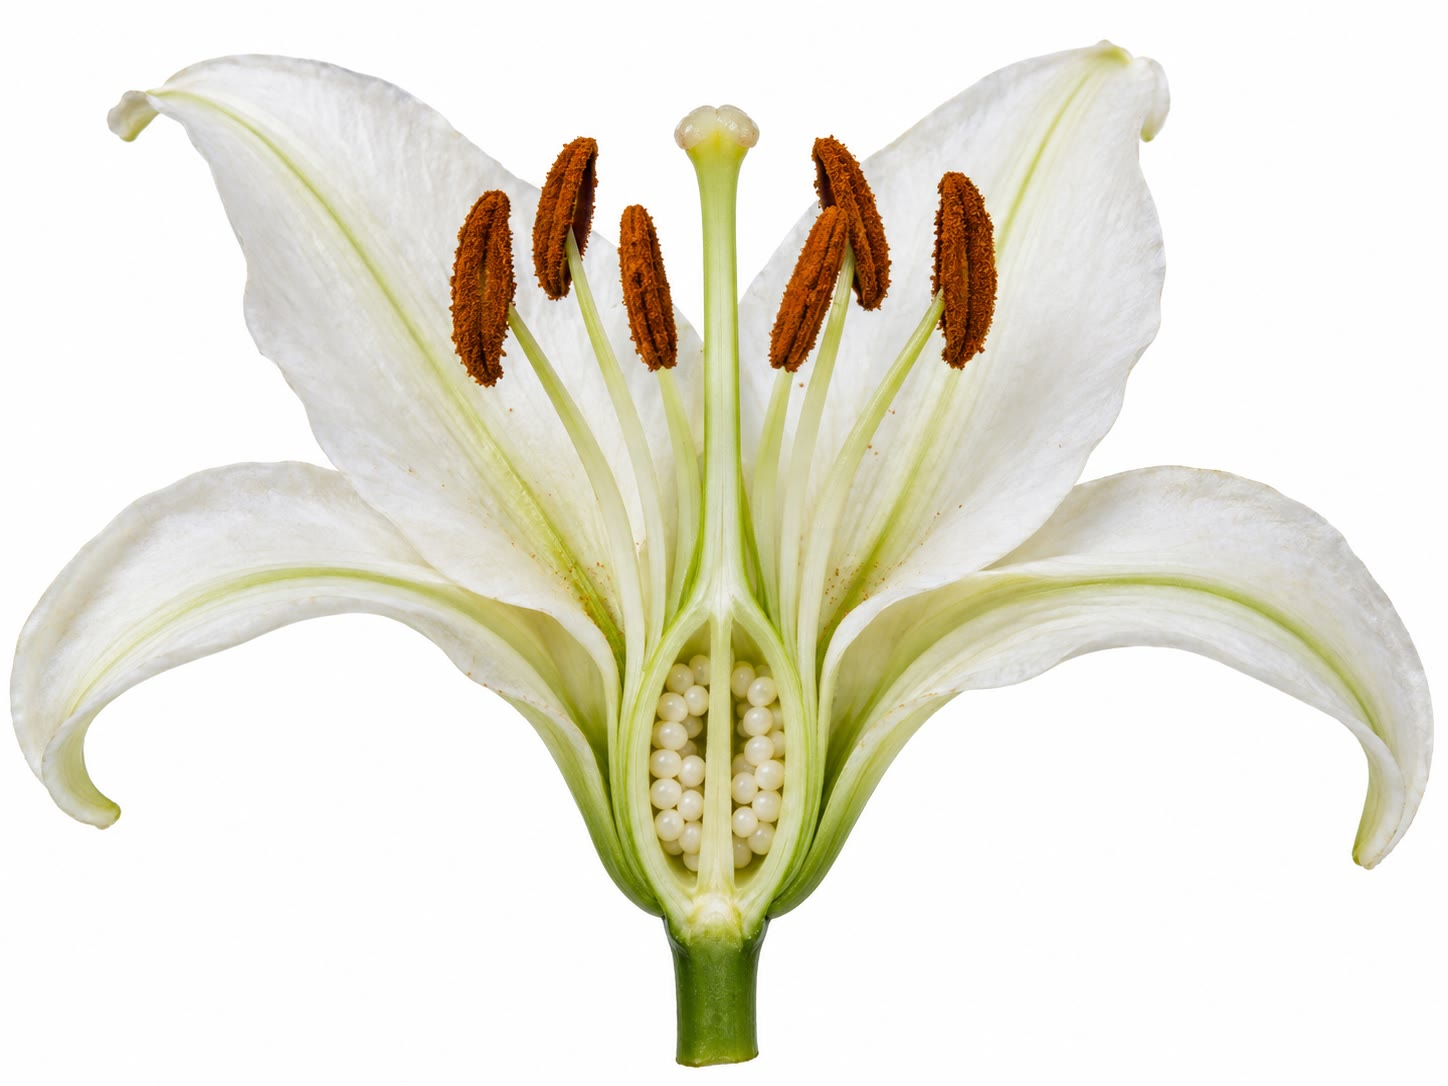
\includegraphics[width=0.55\linewidth]{images/book4/ai/b4-06-lily-dissected.jpg}

{\small A lily cut lengthwise: six \omterm{def:b2:angiosperm-reproduction:flower}{stamens} with pollen-laden
anthers, the long style with its sticky \omterm{def:b2:angiosperm-reproduction:flower}{stigma}, and the \omterm{def:b2:angiosperm-reproduction:flower}{ovary} opened
to show the rows of \omterm{def:b2:plant-life-cycles:heterospory}{ovules}.}
\end{omfigure}

\section{The two gametophytes}

\begin{proposition}[Pollen: the male gametophyte]\label{prop:b2:angiosperm-reproduction:pollen}
\index{pollen grain}\index{microsporogenesis}\index{sporopollenin}
In each \omterm{def:b2:plant-life-cycles:heterospory}{pollen} sac, \omterm{def:b2:meiosis-heredity:meiosis}{diploid} mother cells undergo \omterm{def:b2:meiosis-heredity:meiosis}{meiosis} to give
tetrads of \emph{\omterm{def:b2:plant-life-cycles:heterospory}{microspores}}. Each \omterm{def:b2:plant-life-cycles:heterospory}{microspore} divides once,
unequally, into a large \emph{vegetative cell} and a small
\emph{generative cell} enclosed within it; the generative cell
divides once more, before or after \omterm{def:b2:angiosperm-reproduction:pollination}{pollination}, into two
\emph{sperm cells}. The mature \emph{\omterm{prop:b2:angiosperm-reproduction:pollen}{pollen grain}} is thus a
three-celled \omterm{def:b2:meiosis-heredity:meiosis}{haploid} organism --- the whole male \omterm{def:b2:plant-life-cycles:cycles}{gametophyte} --- of
\qtyrange{10}{100}{\micro m}, sealed in a wall whose outer layer of
\emph{sporopollenin}, the most resistant biological polymer known,
is sculpted with spines, pores and furrows characteristic of the
species, which is why \omterm{def:b2:plant-life-cycles:heterospory}{pollen} identifies plants in sediments tens of
millions of years old. The grain is shed dehydrated, and survives
hours (grasses) to weeks (some trees) until it reaches a \omterm{def:b2:angiosperm-reproduction:flower}{stigma}.
\end{proposition}

\begin{omfigure}
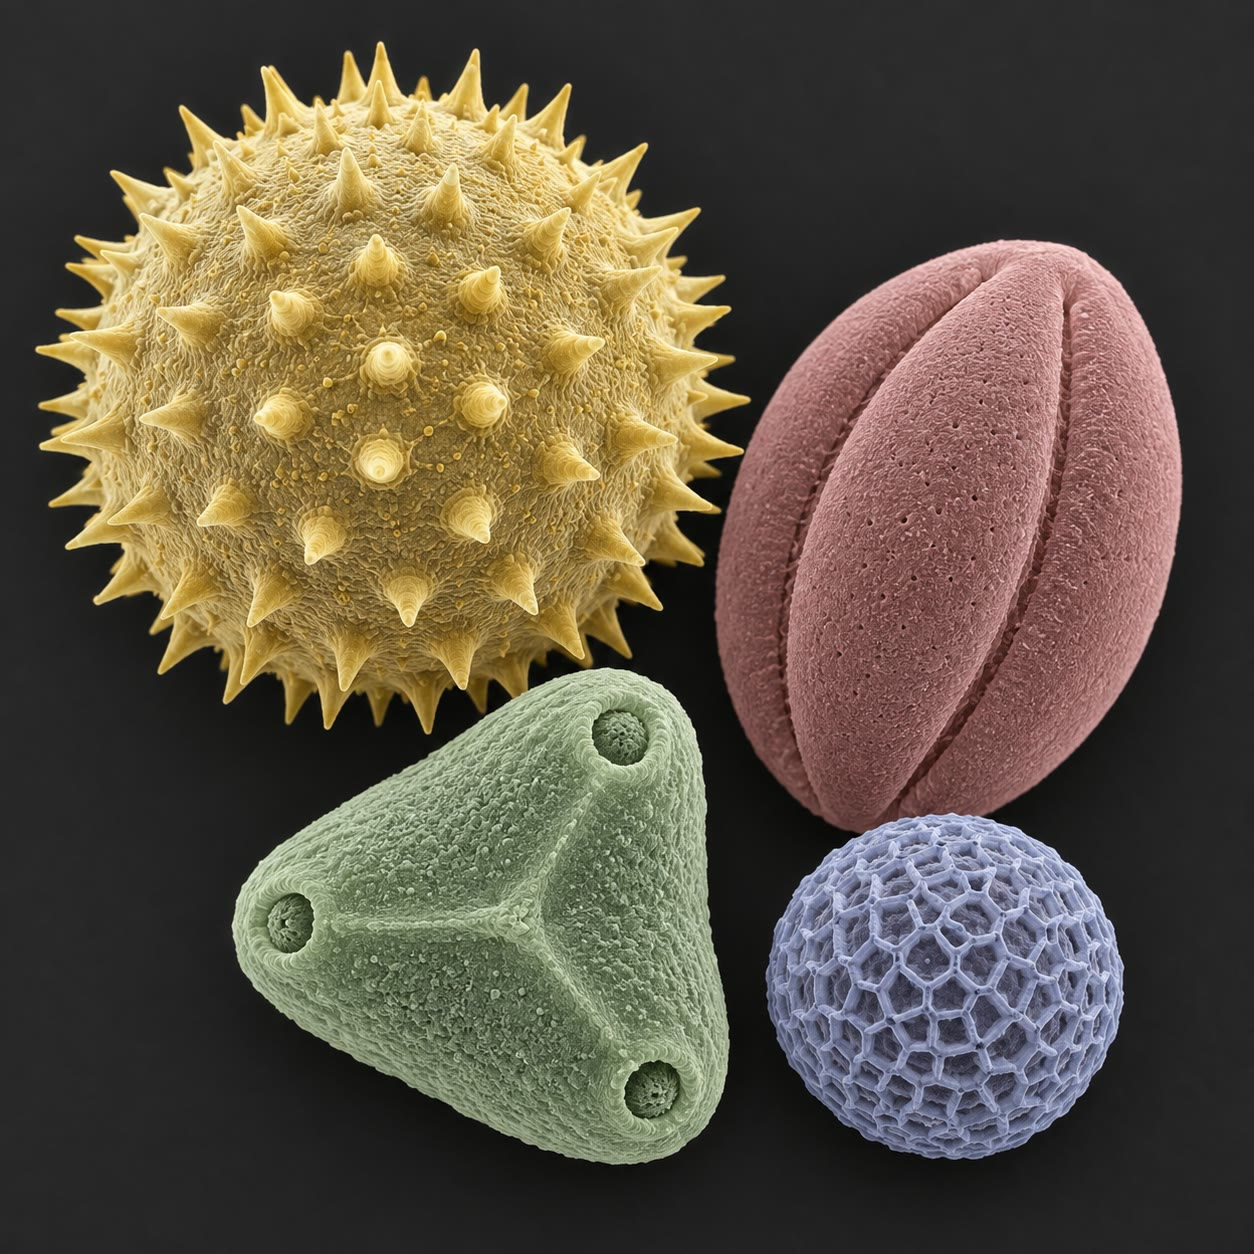
\includegraphics[width=0.45\linewidth]{images/book4/ai/b4-06-pollen-sem.jpg}

{\small \omterm{prop:b2:angiosperm-reproduction:pollen}{Pollen grains} under the scanning electron microscope: the
sporopollenin wall of each species has its own sculpture --- spines,
furrows, pores, a net --- by which it can be recognised.}
\end{omfigure}

\begin{proposition}[The embryo sac: the female gametophyte]\label{prop:b2:angiosperm-reproduction:embryosac}
\index{embryo sac}\index{megasporogenesis}\index{polar nuclei}
In each \omterm{def:b2:plant-life-cycles:heterospory}{ovule}, one \omterm{def:b2:meiosis-heredity:meiosis}{diploid} cell of the nucellus undergoes \omterm{def:b2:meiosis-heredity:meiosis}{meiosis};
three of the four \omterm{def:b2:plant-life-cycles:heterospory}{megaspores} degenerate and the fourth grows, by
three mitoses without cell division, into an eight-nucleate,
seven-celled \emph{\omterm{prop:b2:angiosperm-reproduction:embryosac}{embryo sac}}: at the micropylar end the \emph{egg}
flanked by two \emph{synergids}; at the far end three
\emph{antipodal} cells; in the middle a large \emph{central cell}
containing two \emph{\omterm{prop:b2:angiosperm-reproduction:embryosac}{polar nuclei}}. This sac, wrapped in the nucellus
and two integuments with a micropyle, is the entire female
\omterm{def:b2:plant-life-cycles:cycles}{gametophyte} --- seven cells where a \omterm{def:b2:plant-life-cycles:moss}{moss} had a plant. The two \omterm{prop:b2:angiosperm-reproduction:embryosac}{polar
nuclei} are genetically identical to the egg, a fact that matters for
the endosperm.
\end{proposition}

\begin{omfigure}
\begin{tikzpicture}[every node/.style={font=\scriptsize}]
  % pollen grain
  \begin{scope}
    \draw[very thick, omProp!80!black, fill=omProp!15] (0,0) circle (1.1);
    \draw[thick, omProp!80!black] (0,0) circle (0.95);
    \foreach \a in {0,30,...,330} \draw[omProp!80!black, thick] (\a:1.1) -- (\a:1.25);
    \draw[thick, fill=omDef!25] (0.15,-0.2) ellipse (0.55 and 0.4); \node[font=\tiny] at (0.15,-0.2) {vegetative};
    \draw[thick, fill=omThm!30] (-0.3,0.45) ellipse (0.22 and 0.14); \draw[thick, fill=omThm!30] (0.2,0.5) ellipse (0.22 and 0.14);
    \draw[omThm] (0.0,0.62) -- (0.0,1.5); \node[omThm, anchor=south] at (0.0,1.5) {two sperm cells};
    \node[below, align=center] at (0,-1.4) {pollen grain ($n$)\\3 cells, sporopollenin wall};
  \end{scope}
  % ovule with embryo sac
  \begin{scope}[xshift=5.5cm]
    \draw[thick, fill=omExo!25] (0,0) ellipse (1.5 and 2.1);
    \draw[thick, fill=omExo!10] (0,0) ellipse (1.15 and 1.75);
    \fill[white] (-0.3,1.7) rectangle (0.3,2.2); \draw[thick] (-0.3,1.7) -- (-0.3,2.15); \draw[thick] (0.3,1.7) -- (0.3,2.15);
    \draw[thick, fill=white] (0,0) ellipse (0.7 and 1.35);
    % cells: egg + synergids top, central, antipodals bottom
    \draw[thick, fill=omThm!30] (0,0.95) circle (0.17); \node[omThm, anchor=west] at (1.6,1.2) {egg};
    \draw[thick, fill=omDef!25] (-0.35,1.0) circle (0.14); \draw[thick, fill=omDef!25] (0.35,1.0) circle (0.14); \node[anchor=west] at (1.6,0.75) {two synergids};
    \draw[thick, fill=omDef!10] (0,0) ellipse (0.55 and 0.6); \fill[omDef!80!black] (-0.15,0.05) circle (0.09); \fill[omDef!80!black] (0.15,0.05) circle (0.09);
    \node[anchor=west, align=left] at (1.6,0.1) {central cell with\\two polar nuclei};
    \foreach \x in {-0.3,0,0.3} \draw[thick, fill=omDef!25] (\x,-1.0) circle (0.13); \node[anchor=west] at (1.6,-1.0) {three antipodals};
    \draw (0.35,2.0) -- (1.6,2.0) node[right] {micropyle};
    \draw (1.3,-0.9) -- (1.6,-1.6) node[right] {integuments};
    \draw (0.9,-1.35) -- (1.6,-2.1) node[right] {nucellus};
    \draw (1.6,1.2) -- (0.17,0.95); \draw (1.6,0.75) -- (0.49,1.0); \draw (1.6,0.1) -- (0.55,0.05); \draw (1.6,-1.0) -- (0.43,-1.0);
    \node[below, align=center] at (0,-2.3) {ovule with embryo sac ($n$)\\7 cells, 8 nuclei};
  \end{scope}
\end{tikzpicture}

{\small The two \omterm{def:b2:plant-life-cycles:cycles}{gametophytes} of a flowering plant, both reduced to a
few cells: the three-celled \omterm{prop:b2:angiosperm-reproduction:pollen}{pollen grain}, and the seven-celled
\omterm{prop:b2:angiosperm-reproduction:embryosac}{embryo sac} inside the \omterm{def:b2:plant-life-cycles:heterospory}{ovule}.}
\end{omfigure}

\section{Pollination}

\begin{definition}[Pollination and its agents]\label{def:b2:angiosperm-reproduction:pollination}
\index{pollination}\index{pollination syndrome}\index{nectar}
\emph{Pollination} is the transfer of \omterm{def:b2:plant-life-cycles:heterospory}{pollen} from an anther to a
\omterm{def:b2:angiosperm-reproduction:flower}{stigma}; \emph{self-pollination} within one \omterm{def:b2:angiosperm-reproduction:flower}{flower} or plant,
\emph{cross-pollination} between plants. \emph{Wind-pollinated}
\omterm{def:b2:angiosperm-reproduction:flower}{flowers} (grasses, oaks, birches, plantains) are small, green,
scentless, with large feathery \omterm{def:b2:angiosperm-reproduction:flower}{stigmas} and enormous quantities of
smooth, dry \omterm{def:b2:plant-life-cycles:heterospory}{pollen}; their pollen-to-ovule ratio runs to a million.
\emph{Animal-pollinated} \omterm{def:b2:angiosperm-reproduction:flower}{flowers} pay their carrier: \emph{nectar}
(sugar solution from nectaries), \omterm{def:b2:plant-life-cycles:heterospory}{pollen} itself, oils, scent; and
they advertise with colour, shape and smell tuned to the carrier's
senses --- ultraviolet nectar guides for bees, which see ultraviolet
and not red; red tubular \omterm{def:b2:angiosperm-reproduction:flower}{flowers} without scent for hummingbirds;
white, heavily scented, night-opening \omterm{def:b2:angiosperm-reproduction:flower}{flowers} with deep tubes for
moths; brown, foetid \omterm{def:b2:angiosperm-reproduction:flower}{flowers} for carrion flies; sturdy, pale,
night \omterm{def:b2:angiosperm-reproduction:flower}{flowers} for bats. Each such set of traits is a \emph{pollination
syndrome}, and the fit between \omterm{def:b2:angiosperm-reproduction:flower}{flower} and pollinator is the
textbook case of \emph{coevolution}: Darwin predicted from a
Madagascan orchid's \qty{30}{cm} nectar spur a moth with a
\qty{30}{cm} tongue, found forty years later.
\end{definition}

\begin{omfigure}
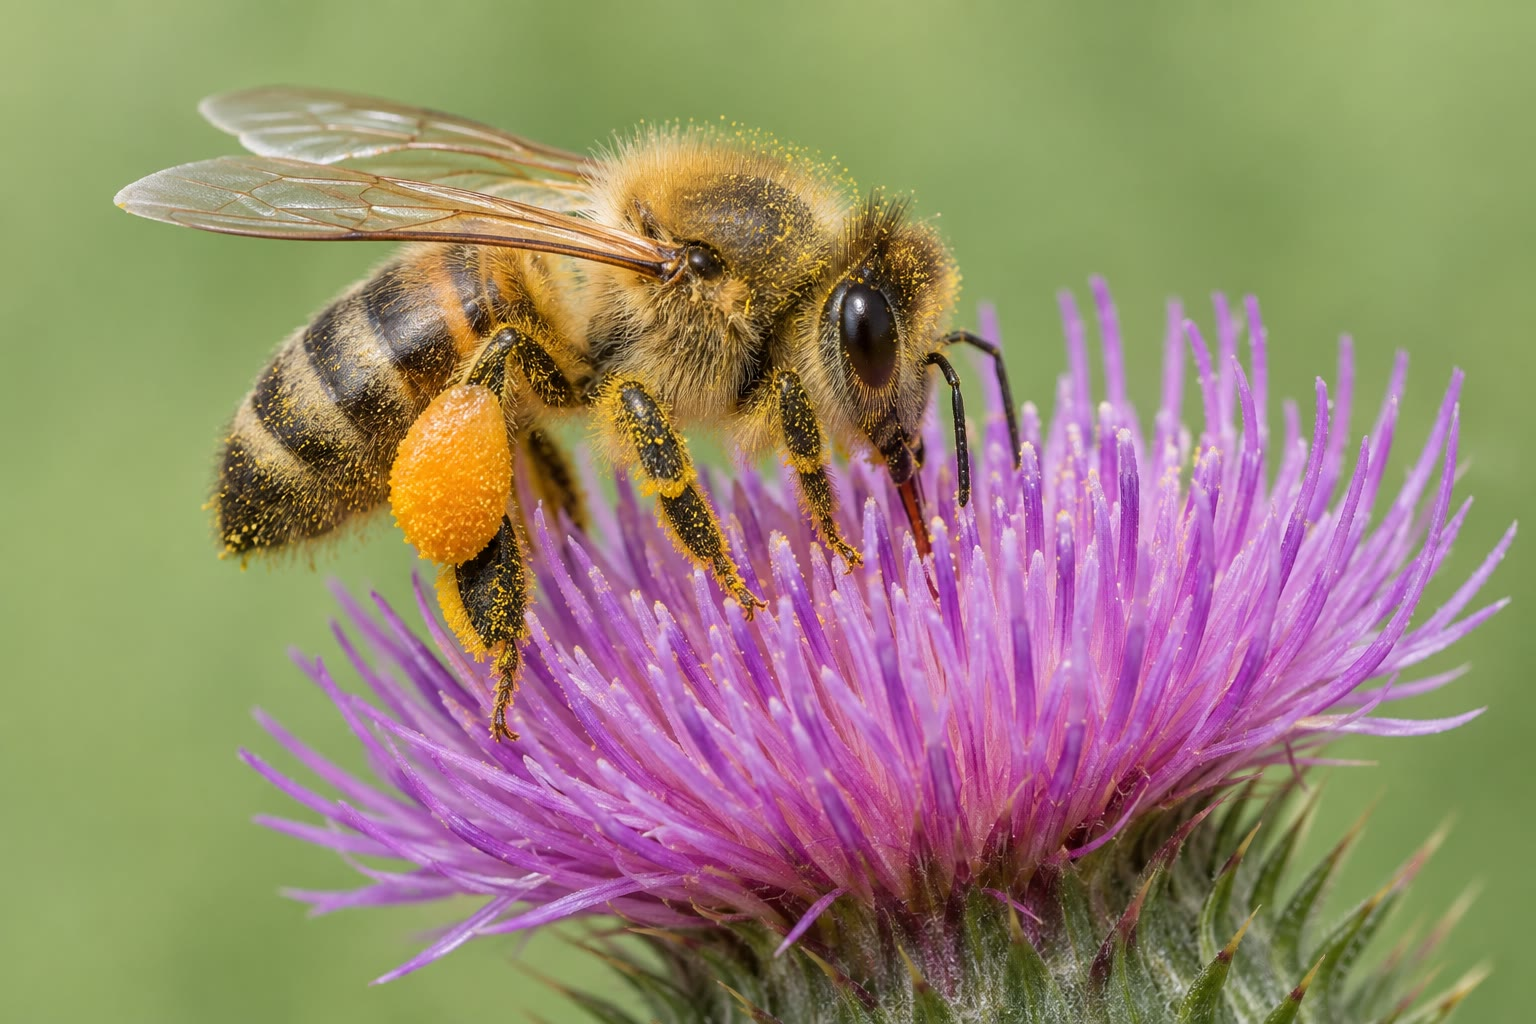
\includegraphics[width=0.58\linewidth]{images/book4/ai/b4-06-bee-on-flower.jpg}

{\small A honeybee on a thistle: \omterm{def:b2:plant-life-cycles:heterospory}{pollen} dusts its body and packs its
hind-leg baskets; some of it will reach the \omterm{def:b2:angiosperm-reproduction:flower}{stigma} of the next
thistle it visits. Purple, a landing platform and abundant \omterm{def:b2:angiosperm-reproduction:pollination}{nectar}
are the bee syndrome.}
\end{omfigure}

\begin{proposition}[Avoiding self-fertilisation]\label{prop:b2:angiosperm-reproduction:selfing}
\index{self-incompatibility}\index{heterostyly}\index{dichogamy}
A hermaphrodite \omterm{def:b2:angiosperm-reproduction:flower}{flower} could fertilise itself, and many do (peas,
wheat, tomatoes); but selfing exposes \omterm{def:b2:meiosis-heredity:vocabulary}{recessive} deleterious \omterm{def:b2:meiosis-heredity:vocabulary}{alleles}
(\emph{inbreeding depression}), and most species prevent it. In time:
\emph{dichogamy}, anthers and \omterm{def:b2:angiosperm-reproduction:flower}{stigma} maturing at different times
(protandry in most umbellifers and composites). In space:
\emph{herkogamy}, anthers and \omterm{def:b2:angiosperm-reproduction:flower}{stigma} held apart, as in the
\emph{heterostyly} of primroses, whose pin \omterm{def:b2:angiosperm-reproduction:flower}{flowers} (long style, low
anthers) and thrum \omterm{def:b2:angiosperm-reproduction:flower}{flowers} (short style, high anthers) place \omterm{def:b2:plant-life-cycles:heterospory}{pollen}
on different parts of an insect. Biochemically:
\emph{self-incompatibility}, a recognition system in which \omterm{def:b2:plant-life-cycles:heterospory}{pollen}
carrying an $S$ \omterm{def:b2:meiosis-heredity:vocabulary}{allele} shared with the pistil is rejected. In
\emph{gametophytic} incompatibility (apples, cherries, petunias,
grasses) the \omterm{def:b2:plant-life-cycles:heterospory}{pollen}'s own \omterm{def:b2:meiosis-heredity:meiosis}{haploid} $S$ \omterm{def:b2:meiosis-heredity:vocabulary}{allele} decides: a pistil
$S_1S_2$ stops $S_1$ and $S_2$ tubes in the style, so that \omterm{def:b2:plant-life-cycles:heterospory}{pollen} from
an $S_1S_3$ plant is half compatible and from $S_3S_4$ wholly. In
\emph{sporophytic} incompatibility (cabbages, sunflowers) the
\omterm{def:b2:meiosis-heredity:meiosis}{diploid} \omterm{def:b2:meiosis-heredity:vocabulary}{genotype} of the \omterm{def:b2:plant-life-cycles:heterospory}{pollen}'s parent decides, on the \omterm{def:b2:angiosperm-reproduction:flower}{stigma}
surface. A rare $S$ \omterm{def:b2:meiosis-heredity:vocabulary}{allele} is compatible with almost every partner,
so selection keeps dozens of \omterm{def:b2:meiosis-heredity:vocabulary}{alleles} in a population.
\end{proposition}
\begin{proof}[Evidence]
Darwin (1862, 1877) crossed primroses by hand: \omterm{def:b2:plant-life-cycles:heterospory}{pollen} from a thrum
\omterm{def:b2:angiosperm-reproduction:flower}{flower} on a pin \omterm{def:b2:angiosperm-reproduction:flower}{stigma} (a ``legitimate'' union) set full capsules;
pin on pin or thrum on thrum (``illegitimate'') set few \omterm{def:b2:angiosperm-reproduction:seed}{seeds} or
none, though the plants were healthy and the \omterm{def:b2:plant-life-cycles:heterospory}{pollen} alive. He
concluded that the two forms were mutually adapted to cross and
protected from selfing, and by counting \omterm{def:b2:angiosperm-reproduction:seed}{seeds} per capsule in
thousands of crosses he measured the cost of self-fertilisation in
dozens of species: selfed offspring were shorter, lighter and less
fertile, generation after generation.
\end{proof}

\begin{omfigure}
\begin{tikzpicture}[every node/.style={font=\scriptsize}]
  % pistil S1S2 with pollen tubes
  \draw[thick, fill=omDef!10] (-0.5,0) rectangle (0.5,3.2);
  \draw[thick, fill=omDef!30] (0,3.3) ellipse (0.7 and 0.2);
  \draw[thick, fill=omDef!12] (0,-0.6) ellipse (0.9 and 0.7);
  \node at (0,-0.6) {ovary};
  \node[anchor=east] at (-1.1,3.3) {stigma of an $S_1S_2$ plant};
  % pollen grains
  \draw[thick, fill=omThm!40] (-0.35,3.75) circle (0.13); \node[omThm, left] at (-0.5,3.75) {$S_1$};
  \draw[thick, fill=omThm!40] (0,3.75) circle (0.13); \node[omThm, anchor=south] at (0,3.92) {$S_2$};
  \draw[thick, fill=omExo!70!black] (0.35,3.75) circle (0.13); \node[right] at (0.5,3.75) {$S_3$};
  % tubes: S1 and S2 stop in the style, S3 reaches the ovary
  \draw[thick, omThm] (-0.35,3.3) -- (-0.35,2.3); \node[omThm, left, align=right] at (-0.55,2.3) {tube $S_1$\\arrested};
  \draw[thick, omThm] (0,3.3) -- (0,2.0);
  \draw[thick, omExo!70!black] (0.35,3.3) -- (0.35,-0.2) -- (0.2,-0.5);
  \node[right, align=left] at (0.55,0.9) {tube $S_3$\\reaches an ovule};
  \node[anchor=west, align=left, text width=6cm] at (3.2,3.2) {gametophytic self-incompatibility: a pollen tube whose own $S$ allele matches either allele of the pistil is stopped in the style};
  \node[anchor=west, align=left, text width=6cm] at (3.2,1.4) {pollen from an $S_1S_2$ plant: 0 compatible\\from $S_1S_3$: half\\from $S_3S_4$: all};
\end{tikzpicture}

{\small Gametophytic self-incompatibility. On an $S_1S_2$ pistil,
tubes carrying $S_1$ or $S_2$ are arrested in the style; an $S_3$
tube grows to the \omterm{def:b2:angiosperm-reproduction:flower}{ovary}.}
\end{omfigure}

\section{Fertilisation}

\begin{theorem}[The pollen tube]\label{thm:b2:angiosperm-reproduction:tube}
\index{pollen tube}
A \omterm{prop:b2:angiosperm-reproduction:pollen}{pollen grain} on a compatible \omterm{def:b2:angiosperm-reproduction:flower}{stigma} rehydrates and grows a
\emph{\omterm{thm:b2:angiosperm-reproduction:tube}{pollen tube}}: the vegetative cell extends by tip growth,
laying down new wall at the apex at a rate of \qtyrange{0.1}{1}{cm/h},
digesting its way through the transmitting tissue of the style and
feeding on it. The tube carries the two sperm cells at its tip; it
is guided the last distance by peptides secreted by the synergids,
enters the \omterm{def:b2:plant-life-cycles:heterospory}{ovule} through the micropyle, bursts into one synergid,
and releases the sperm. A tube crossing a style of length $L$ at
speed $v$ takes $L/v$: a few hours in a cherry, a full day in maize,
whose ``silks'' are styles \qty{20}{cm} long. \omterm{def:b2:plant-life-cycles:heterospory}{Pollen} viability sets
a clock: grass \omterm{def:b2:plant-life-cycles:heterospory}{pollen} dies in hours, so a \omterm{def:b2:angiosperm-reproduction:flower}{stigma} must be reached
quickly.
\end{theorem}
\begin{proof}
The time is the length divided by the growth rate; for maize,
\qty{20}{cm} at \qty{1}{cm/h} gives \qty{20}{h}. The tube itself
consists almost entirely of wall and a thin film of cytoplasm behind
the tip, so that the vegetative cell's reserves, plus what it
absorbs from the style, suffice for a length a thousand times the
grain's diameter.
\end{proof}

\begin{proposition}[Double fertilisation]\label{prop:b2:angiosperm-reproduction:double}
\index{double fertilisation}\index{endosperm}
Of the two sperm cells delivered by the tube, one fuses with the
egg to form the \omterm{def:b2:meiosis-heredity:meiosis}{diploid} \emph{zygote}, from which the embryo grows;
the other fuses with the central cell and its two \omterm{prop:b2:angiosperm-reproduction:embryosac}{polar nuclei} to
form a \emph{triploid} nucleus ($3n$: two maternal genomes, one
paternal), from which the \emph{endosperm} grows --- a nutritive
tissue that fills the \omterm{def:b2:angiosperm-reproduction:seed}{seed} with starch, oil and protein. Both
fertilisations happen within minutes of each other; neither
succeeds without the other in most species, so that a plant
provisions only those \omterm{def:b2:angiosperm-reproduction:seed}{seeds} that carry an embryo. The endosperm is
the tissue that feeds humanity: the flour of wheat and rice, the
meal of maize, the white of a coconut are triploid endosperm. In
gymnosperms the \omterm{def:b2:angiosperm-reproduction:seed}{seed}'s food store is the female \omterm{def:b2:plant-life-cycles:cycles}{gametophyte}, built
before fertilisation whether or not an embryo follows; the
angiosperm's endosperm is made to order.
\end{proposition}
\begin{proof}[Evidence]
Nawaschin (1898), following the \omterm{thm:b2:angiosperm-reproduction:tube}{pollen tube} of a lily and a
fritillary into the \omterm{prop:b2:angiosperm-reproduction:embryosac}{embryo sac} under the microscope, saw both sperm
nuclei leave the tube, one entering the egg and the other fusing
with the \omterm{prop:b2:angiosperm-reproduction:embryosac}{polar nuclei}; Guignard confirmed it the next year in other
species. The triploidy of the endosperm followed from chromosome
counts, and its genetic consequences --- a kernel's endosperm
showing the \omterm{def:b2:plant-life-cycles:heterospory}{pollen} parent's traits (\emph{xenia}), in the ratio two
maternal doses to one paternal --- had been noticed by breeders of
maize long before.
\end{proof}

\begin{omfigure}
\begin{tikzpicture}[every node/.style={font=\scriptsize}, >=stealth]
  \node[draw, rounded corners, fill=omProp!15, align=center] (sp) at (0,2) {sperm cell 1 ($n$)};
  \node[draw, rounded corners, fill=omProp!15, align=center] (sp2) at (0,0) {sperm cell 2 ($n$)};
  \node[draw, rounded corners, fill=omThm!15, align=center] (egg) at (4,2) {egg ($n$)};
  \node[draw, rounded corners, fill=omDef!15, align=center] (cc) at (4,0) {central cell\\two polar nuclei ($n + n$)};
  \node[draw, rounded corners, fill=omThm!30, align=center] (zyg) at (8.6,2) {zygote ($2n$)\\$\to$ embryo};
  \node[draw, rounded corners, fill=omDef!30, align=center] (endo) at (8.6,0) {endosperm nucleus ($3n$)\\$\to$ endosperm, the food store};
  \draw[->, thick] (sp) -- (egg); \draw[->, thick] (egg) -- (zyg);
  \draw[->, thick] (sp2) -- (cc); \draw[->, thick] (cc) -- (endo);
  \node[anchor=south] at (2,2.5) {fertilisation 1};
  \node[anchor=south] at (2,0.5) {fertilisation 2};
  \node[anchor=north, align=center] at (4.3,-0.9) {one pollen tube, two sperm cells, two fusions: the embryo and its food supply are made together};
\end{tikzpicture}

{\small \omterm{prop:b2:angiosperm-reproduction:double}{Double fertilisation}: one sperm makes the \omterm{def:b2:meiosis-heredity:meiosis}{diploid} zygote,
the other the triploid endosperm.}
\end{omfigure}

\section{Seed and fruit}

\begin{definition}[From ovule to seed, from ovary to fruit]\label{def:b2:angiosperm-reproduction:seed}
\index{seed}\index{fruit}\index{cotyledon}\index{dormancy}
The zygote divides into a suspensor, which pushes the embryo into
the endosperm, and an embryo proper that passes through globular,
heart and torpedo stages as it lays down the root and shoot poles
and one or two \emph{cotyledons} (seed leaves) --- the monocot--dicot
distinction. In many dicots (beans, peas) the growing cotyledons
absorb the endosperm and become the food store themselves; in
cereals and most monocots the endosperm persists and the single
cotyledon is a sucking organ. The integuments harden into the
\emph{seed coat}; the seed dehydrates to \qtyrange{5}{15}{\%} water,
metabolism stops, and it enters \emph{dormancy}, which ends only
when a signal --- water, cold, light, fire, the passage through a
gut --- says the season is right. Meanwhile the \omterm{def:b2:angiosperm-reproduction:flower}{ovary} wall grows into
the \emph{fruit}, whose form is a dispersal strategy: dry fruits
that split (pods, capsules) or do not (grains, nuts, winged
samaras), fleshy fruits that are eaten (berries, drupes with a stone,
the apple, whose flesh is receptacle); the seed passes through the
animal unharmed, its coat scarified, and is deposited with fertiliser
kilometres away.
\end{definition}
\begin{proof}[Evidence]
The cereal grain shows how germination is controlled. The embryo,
on imbibing water, secretes gibberellin into the surrounding
endosperm; the outer layer of the endosperm, the aleurone, responds
by making and secreting $\alpha$-amylase, which digests the starch
into sugars the embryo absorbs. Half-grains without an embryo make no
amylase; add gibberellin to them and they do (Paleg, Yomo, 1960); the
hormone acts by switching on the amylase gene, one of the first cases
in which a plant hormone was traced to a gene. Brewers have used the
process for millennia: malting is barley made to germinate and then
dried.
\end{proof}

\begin{omfigure}
\begin{tikzpicture}[every node/.style={font=\scriptsize}]
  % embryogenesis stages
  \foreach \x/\lab in {0/{zygote}, 1.6/{two cells}, 3.4/{globular}, 5.6/{heart}, 8.2/{torpedo}} \node[below] at (\x,-1.1) {\lab};
  \draw[thick, fill=omThm!25] (0,-0.2) circle (0.22);
  \draw[thick, fill=omThm!25] (1.6,0.0) circle (0.2); \draw[thick, fill=omDef!15] (1.6,-0.45) circle (0.14);
  \draw[thick, fill=omThm!25] (3.4,0.1) circle (0.45); \foreach \y in {-0.5,-0.75,-1.0} \draw[thick, fill=omDef!15] (3.4,\y) circle (0.1);
  \draw[thick, fill=omThm!25] (5.6,0.0) .. controls (4.9,1.0) and (5.2,-0.6) .. (5.6,-0.6) .. controls (6.0,-0.6) and (6.3,1.0) .. (5.6,0.0);
  \draw[thick, fill=omThm!25] (5.15,0.5) circle (0.32); \draw[thick, fill=omThm!25] (6.05,0.5) circle (0.32);
  \foreach \y in {-0.75,-1.0} \draw[thick, fill=omDef!15] (5.6,\y) circle (0.09);
  \draw[thick, fill=omThm!25] (8.2,-0.2) ellipse (0.3 and 0.75);
  \draw[thick, fill=omThm!25] (7.75,0.9) .. controls (7.4,1.6) and (7.9,1.9) .. (8.05,0.55) -- cycle;
  \draw[thick, fill=omThm!25] (8.65,0.9) .. controls (9.0,1.6) and (8.5,1.9) .. (8.35,0.55) -- cycle;
  \node[omDef!80!black, anchor=west] at (9.3,-0.9) {suspensor (blue)};
  \node[omThm, anchor=west] at (9.3,0.9) {cotyledons};
  \node[anchor=west] at (9.3,-0.2) {root pole below};
\end{tikzpicture}

{\small Embryogenesis in a dicot: the zygote divides into an embryo
and a suspensor; the globular embryo becomes heart-shaped as the two
\omterm{def:b2:angiosperm-reproduction:seed}{cotyledons} emerge, then torpedo-shaped as the root--shoot axis
extends.}
\end{omfigure}

\begin{omfigure}
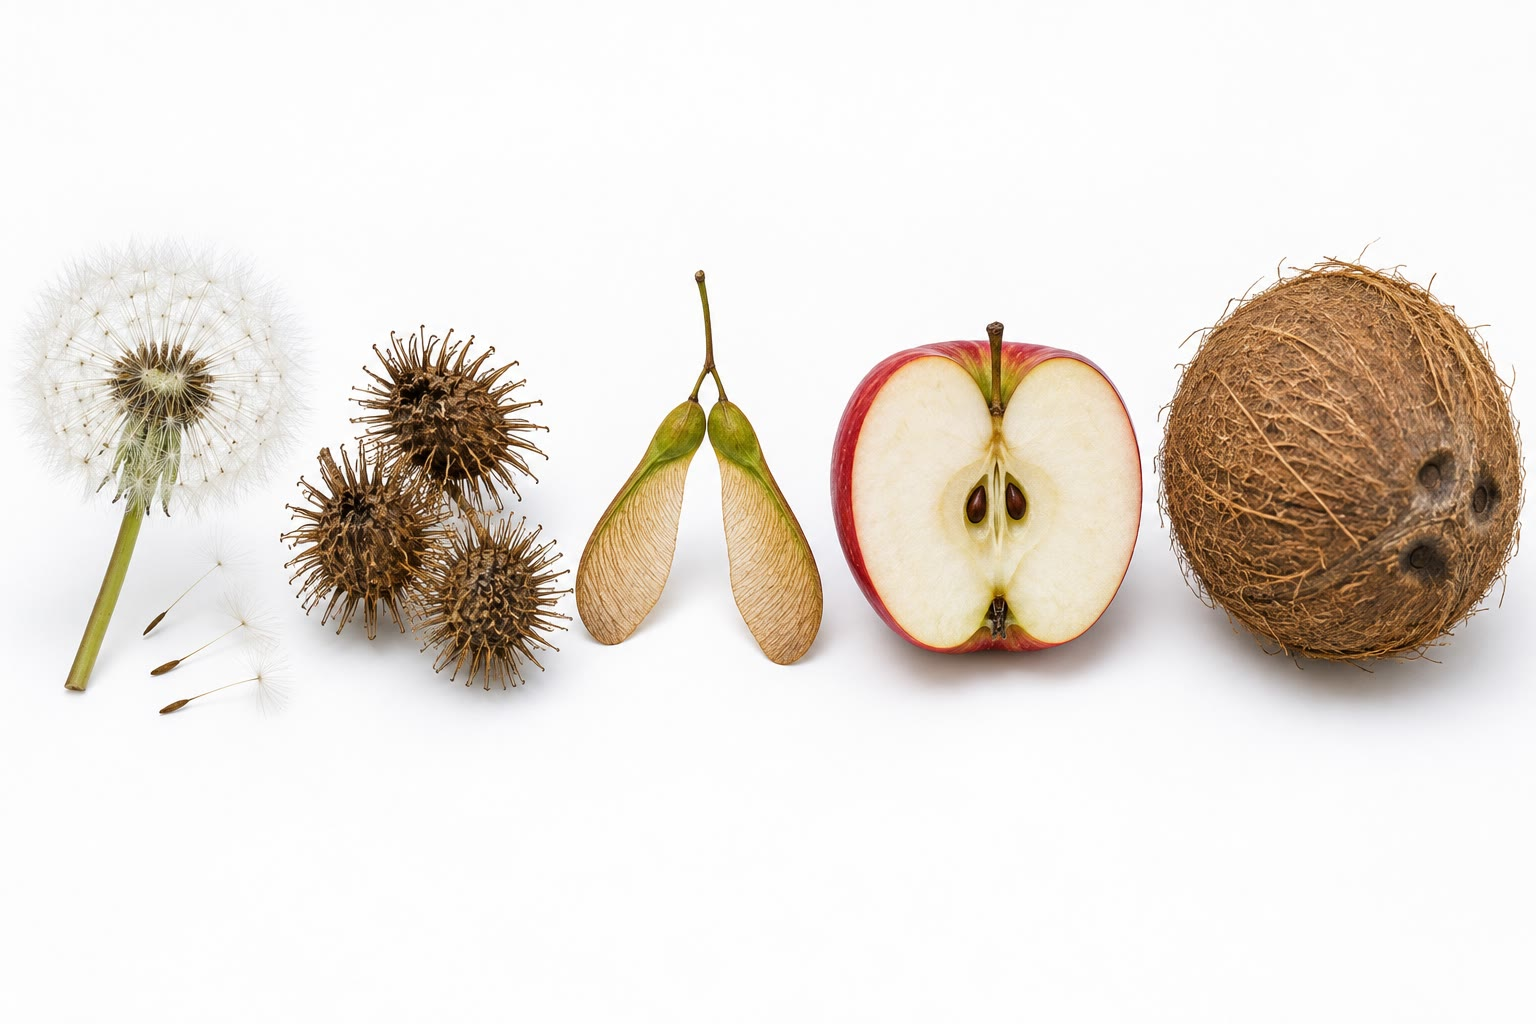
\includegraphics[width=0.62\linewidth]{images/book4/ai/b4-06-fruits-seeds.jpg}

{\small \omterm{def:b2:angiosperm-reproduction:seed}{Fruits} built for dispersal: parachutes (dandelion), hooks
(burdock), wings (maple), flesh for an animal (apple), and a buoyant
husk for the sea (coconut).}
\end{omfigure}

\begin{example}[Dispersal distances]\label{ex:b2:angiosperm-reproduction:dispersal}
A dandelion achene with its parachute descends at \qty{0.3}{m/s};
from \qty{0.3}{m} in a \qty{3}{m/s} wind it flies \qty{3}{m}, and in
a thermal, hundreds. A maple samara autorotates down at
\qty{1}{m/s} from \qty{15}{m}: \qty{45}{m}. A cherry stone dropped by
a bird after a twenty-minute flight at \qty{10}{m/s}: up to
\qty{12}{km}. An oak's acorns fall at its foot unless a jay carries
them, which it does by the thousand, a kilometre and more, and
forgets a tenth of them: the oaks that recolonised Europe after the
last ice age moved north at hundreds of metres a year, far faster
than an acorn rolls, and it was the birds that moved them.
\end{example}

\section{Exercises}

\begin{exercise}[$\star$]\label{exo:b2:angiosperm-reproduction:1}
Name the four whorls of a \omterm{def:b2:angiosperm-reproduction:flower}{flower} and the parts of a \omterm{def:b2:angiosperm-reproduction:flower}{stamen} and of a
\omterm{def:b2:angiosperm-reproduction:flower}{carpel}. Which parts are \omterm{def:b2:meiosis-heredity:meiosis}{diploid} \omterm{def:b2:plant-life-cycles:cycles}{sporophyte}, which are \omterm{def:b2:meiosis-heredity:meiosis}{haploid}
\omterm{def:b2:plant-life-cycles:cycles}{gametophyte}?
\end{exercise}

\begin{exercise}[$\star$]\label{exo:b2:angiosperm-reproduction:2}
Give the ploidy of: a \omterm{def:b2:plant-life-cycles:heterospory}{microspore}, the vegetative cell, a sperm cell,
the egg, a polar nucleus, the zygote, the endosperm, the \omterm{def:b2:angiosperm-reproduction:seed}{seed coat},
the \omterm{def:b2:angiosperm-reproduction:seed}{fruit} wall.
\end{exercise}

\begin{exercise}[$\star$]\label{exo:b2:angiosperm-reproduction:3}
List five traits of a wind-pollinated \omterm{def:b2:angiosperm-reproduction:flower}{flower} and five of a
bee-pollinated one, and give a plant for each.
\end{exercise}

\begin{exercise}[$\star$]\label{exo:b2:angiosperm-reproduction:4}
What is \omterm{prop:b2:angiosperm-reproduction:double}{double fertilisation}, and what is made by each of the two
fusions? Why can the endosperm be called ``made to order''?
\end{exercise}

\begin{exercise}[$\star\star$]\label{exo:b2:angiosperm-reproduction:5}
A maize silk is \qty{25}{cm} long and a \omterm{thm:b2:angiosperm-reproduction:tube}{pollen tube} grows at
\qty{1.2}{cm/h}. How long does fertilisation take after \omterm{def:b2:angiosperm-reproduction:pollination}{pollination}?
A tassel sheds \omterm{def:b2:plant-life-cycles:heterospory}{pollen} from day 0 to day 7 and the plant's silks
emerge from day 5 to day 12, one seventh of them each day; a silk
catches \omterm{def:b2:plant-life-cycles:heterospory}{pollen} only while \omterm{def:b2:plant-life-cycles:heterospory}{pollen} is shed. What fraction of the
silks is pollinated?
\end{exercise}

\begin{exercise}[$\star\star$]\label{exo:b2:angiosperm-reproduction:6}
Under gametophytic self-incompatibility, what fraction of \omterm{def:b2:plant-life-cycles:heterospory}{pollen} is
compatible in the crosses $S_1S_2\times S_1S_2$, $S_1S_2\times
S_1S_3$, $S_1S_2\times S_3S_4$ (pistil listed first)? Give the
\omterm{def:b2:meiosis-heredity:vocabulary}{genotypes} of the offspring of the second cross.
\end{exercise}

\begin{exercise}[$\star\star$]\label{exo:b2:angiosperm-reproduction:7}
In a population with $n$ equally frequent $S$ \omterm{def:b2:meiosis-heredity:vocabulary}{alleles}, what fraction
of random \omterm{def:b2:plant-life-cycles:heterospory}{pollen} is compatible with a given plant? Explain why a new
$S$ \omterm{def:b2:meiosis-heredity:vocabulary}{allele} arising by \omterm{def:b2:genome-diversification:mutation}{mutation} spreads, and what this predicts for
the number of \omterm{def:b2:meiosis-heredity:vocabulary}{alleles}.
\end{exercise}

\begin{exercise}[$\star\star$]\label{exo:b2:angiosperm-reproduction:8}
A maize plant \omterm{def:b2:meiosis-heredity:vocabulary}{heterozygous} $Yy$ (yellow endosperm \omterm{def:b2:meiosis-heredity:vocabulary}{dominant}) is
selfed. Give the endosperm \omterm{def:b2:meiosis-heredity:vocabulary}{genotypes} of its kernels and their
proportions, remembering that the two \omterm{prop:b2:angiosperm-reproduction:embryosac}{polar nuclei} are identical.
What fraction of kernels are yellow? What if the plant is pollinated
by a $yy$ plant?
\end{exercise}

\begin{exercise}[$\star\star$]\label{exo:b2:angiosperm-reproduction:9}
Describe the aleurone experiment and explain what it shows about
(a) the role of the embryo, (b) the role of gibberellin, (c) the
site of amylase synthesis. Why is a half-grain without an embryo the
essential control?
\end{exercise}

\begin{exercise}[$\star\star\star$]\label{exo:b2:angiosperm-reproduction:10}
Compare the wind and animal strategies in cost: a wind-pollinated
plant makes $10^{6}$ grains per \omterm{def:b2:plant-life-cycles:heterospory}{ovule} at \qty{1}{\micro g} each; an
animal-pollinated plant makes $10^{3}$ grains per \omterm{def:b2:plant-life-cycles:heterospory}{ovule} at
\qty{1}{\micro g} each plus \qty{5}{mg} of \omterm{def:b2:angiosperm-reproduction:pollination}{nectar} sugar per \omterm{def:b2:angiosperm-reproduction:flower}{flower}
of ten \omterm{def:b2:plant-life-cycles:heterospory}{ovules}. Compute the reproductive cost per \omterm{def:b2:plant-life-cycles:heterospory}{ovule} in each case
(take \omterm{def:b2:plant-life-cycles:heterospory}{pollen} and sugar at the same energy per gram), and explain why
wind \omterm{def:b2:angiosperm-reproduction:pollination}{pollination} nevertheless persists.
\end{exercise}

\begin{exercise}[$\star\star\star$]\label{exo:b2:angiosperm-reproduction:11}
Explain, with the numbers of \cref{ex:b2:angiosperm-reproduction:dispersal},
why a fleshy \omterm{def:b2:angiosperm-reproduction:seed}{fruit} is worth its cost to a tree even though the
animal digests the flesh and drops most \omterm{def:b2:angiosperm-reproduction:seed}{seeds} where they cannot
grow.
\end{exercise}

\begin{exercise}[$\star\star\star$]\label{exo:b2:angiosperm-reproduction:12}
``The closed \omterm{def:b2:angiosperm-reproduction:flower}{carpel} is the reason flowering plants dominate the
land.'' Discuss: what the enclosure of the \omterm{def:b2:plant-life-cycles:heterospory}{ovule} makes possible
(choice of \omterm{def:b2:plant-life-cycles:heterospory}{pollen}, incompatibility, the \omterm{def:b2:angiosperm-reproduction:seed}{fruit}) and what it costs.
\end{exercise}

\section{Problem: An Orchard and a Field}

\begin{problem}[{Weekend problem --- an apple orchard's pollination
planned around self-incompatibility, and a maize field's
fertilisation and yield computed from the pollen it makes, ending on
the orchard's fruit set and the field's kernel count}]
\label{pb:b2:angiosperm-reproduction:1}
Apple is gametophytically self-incompatible. An orchard has three
varieties: A ($S_1S_2$), B ($S_1S_3$), C ($S_3S_4$). A \omterm{def:b2:angiosperm-reproduction:flower}{flower} has five
\omterm{def:b2:angiosperm-reproduction:flower}{carpels} with two \omterm{def:b2:plant-life-cycles:heterospory}{ovules} each, and a \omterm{def:b2:angiosperm-reproduction:seed}{fruit} that sets fewer than five
\omterm{def:b2:angiosperm-reproduction:seed}{seeds} is dropped by the tree. A bee visit deposits \num{100} \omterm{prop:b2:angiosperm-reproduction:pollen}{pollen
grains} on a \omterm{def:b2:angiosperm-reproduction:flower}{stigma}; each compatible grain has probability $0.1$ of
fertilising an \omterm{def:b2:plant-life-cycles:heterospory}{ovule} not yet taken. A tree bears \num{5000} \omterm{def:b2:angiosperm-reproduction:flower}{flowers}
and needs \num{250} \omterm{def:b2:angiosperm-reproduction:seed}{fruits} for a full crop. Maize: a tassel sheds
$10^{7}$ grains over \num{7} days; the field holds \num{8} plants per
square metre; a plant bears one ear of \num{600} silks; a silk
presents \qty{1e-4}{m^2} to falling \omterm{def:b2:plant-life-cycles:heterospory}{pollen}; \omterm{def:b2:plant-life-cycles:heterospory}{pollen} settles at
\qty{0.25}{m/s}; a kernel holds \qty{0.3}{g} of endosperm.

\medskip
\noindent\textbf{Part I --- Compatibility.}
\begin{enumerate}
  \item For \omterm{def:b2:plant-life-cycles:heterospory}{pollen} of each variety on a pistil of A, give the
        compatible fraction $f$.
  \item Same for pistils of B and of C.
  \item A bee arriving from a tree of B deposits 100 grains on an A
        \omterm{def:b2:angiosperm-reproduction:flower}{stigma}: how many are compatible, and how many \omterm{def:b2:plant-life-cycles:heterospory}{ovules} are
        expected to be fertilised (ignore saturation)?
  \item Same for a bee from C, and from another A.
  \item Which \omterm{def:b2:angiosperm-reproduction:seed}{fruits} are kept? What is the risk of planting an
        orchard of variety A alone?
  \item A block of A trees is surrounded by C trees; half the bee
        visits to A come from C. If each \omterm{def:b2:angiosperm-reproduction:flower}{flower} receives one visit,
        what fraction of A \omterm{def:b2:angiosperm-reproduction:flower}{flowers} set \omterm{def:b2:angiosperm-reproduction:seed}{fruit}, and how many \omterm{def:b2:angiosperm-reproduction:seed}{fruits}
        per tree? Is the crop full?
  \item Why do orchards interplant a crab-apple that flowers for
        weeks, and why must its $S$ \omterm{def:b2:meiosis-heredity:vocabulary}{alleles} be checked?
\end{enumerate}

\medskip
\noindent\textbf{Part II --- \omterm{def:b2:plant-life-cycles:heterospory}{Pollen} over the maize field.}
\begin{enumerate}[resume]
  \item Compute the \omterm{def:b2:plant-life-cycles:heterospory}{pollen} released per square metre of field per
        second, on average over the seven days.
  \item At steady state the flux of settling \omterm{def:b2:plant-life-cycles:heterospory}{pollen} equals the
        release rate. Compute the \omterm{def:b2:plant-life-cycles:heterospory}{pollen} concentration in the air
        (grains per cubic metre).
  \item Compute the number of grains landing on one silk per second,
        and the mean waiting time for the first grain.
  \item How many grains does a silk receive in a day? Why is only the
        first useful?
  \item A silk of \qty{20}{cm} is pollinated; the tube grows at
        \qty{1}{cm/h}. When is the \omterm{def:b2:plant-life-cycles:heterospory}{ovule} fertilised?
  \item A drought delays silk emergence by five days while the
        tassel sheds on schedule. Using the seven-day shedding
        period, estimate the fraction of the \omterm{def:b2:plant-life-cycles:heterospory}{pollen} season the silks
        catch, and the consequence for yield.
\end{enumerate}

\medskip
\noindent\textbf{Part III --- \omterm{prop:b2:angiosperm-reproduction:double}{Double fertilisation} and the kernel.}
The field is a variety with yellow endosperm ($Y$, \omterm{def:b2:meiosis-heredity:vocabulary}{dominant}) next to
a white ($yy$) field; the wind blows from the white field.
\begin{enumerate}[resume]
  \item Give the \omterm{def:b2:meiosis-heredity:vocabulary}{genotypes} of the embryo and the endosperm of a
        kernel of a $YY$ plant fertilised by $yy$ \omterm{def:b2:plant-life-cycles:heterospory}{pollen}.
  \item Is the kernel yellow or white? Explain the term xenia.
  \item A $Yy$ plant is pollinated by $yy$ \omterm{def:b2:plant-life-cycles:heterospory}{pollen}: give the endosperm
        \omterm{def:b2:meiosis-heredity:vocabulary}{genotypes} and their frequencies.
  \item The endosperm contains two maternal and one paternal genome.
        A gene with a dosage effect gives, per copy, \qty{10}{units} of
        pigment: what pigment do the kernels $YYy$, $Yyy$ and $yyY$
        (two paternal doses hypothetically) carry? Which of these
        can actually exist?
  \item Explain why the endosperm, not the embryo, is what we eat,
        and what fraction of the kernel's mass it represents if the
        embryo weighs \qty{0.03}{g}.
  \item Why is the endosperm's ``made to order'' provisioning an
        advantage over the gymnosperm's?
\end{enumerate}

\medskip
\noindent\textbf{Part IV --- Yield.}
\begin{enumerate}[resume]
  \item If \qty{90}{\%} of silks are fertilised, compute the kernels
        per ear, per plant and per square metre, and the endosperm
        mass per square metre.
  \item Convert to tonnes per hectare.
  \item The crop fixes \qty{1.2}{kg} of carbon per square metre per
        season, of which half ends in the harvested grain. Check the
        consistency with the mass of question 20 (endosperm is
        \qty{45}{\%} carbon).
  \item How many \omterm{prop:b2:angiosperm-reproduction:pollen}{pollen grains} did the field shed per kernel
        harvested?
  \item Explain why a lone maize plant in a garden sets a poorly
        filled ear.
  \item State the result: the \omterm{def:b2:angiosperm-reproduction:seed}{fruit} set of the A block and the
        field's yield in kernels per square metre and tonnes per
        hectare.
\end{enumerate}
\end{problem}
